Machine vision systems have often been approached with the current fast technology development and intelligent systems. They are used for the most diverse segments, such as the military and medical areas. Image processing has quickly gaining ground. For instance, this is essential when comes to finding a pattern or extract a specific feature in an image. 

Colored or gray scaled images can be treated as matrices with dimensions given by their pixel resolution. Each pixel corresponds to a cell inside this matrix and each cell contains a relevant information, which could be a level in grayscale, a coordinate or a temperature as in this paper. Since they are matrices, they can be easily manipulated by means of mathematical operations and consequently processed to highlight one specific property or more.

\begin{figure}[H]
	\centering
	\captionsetup{justification=centering}
	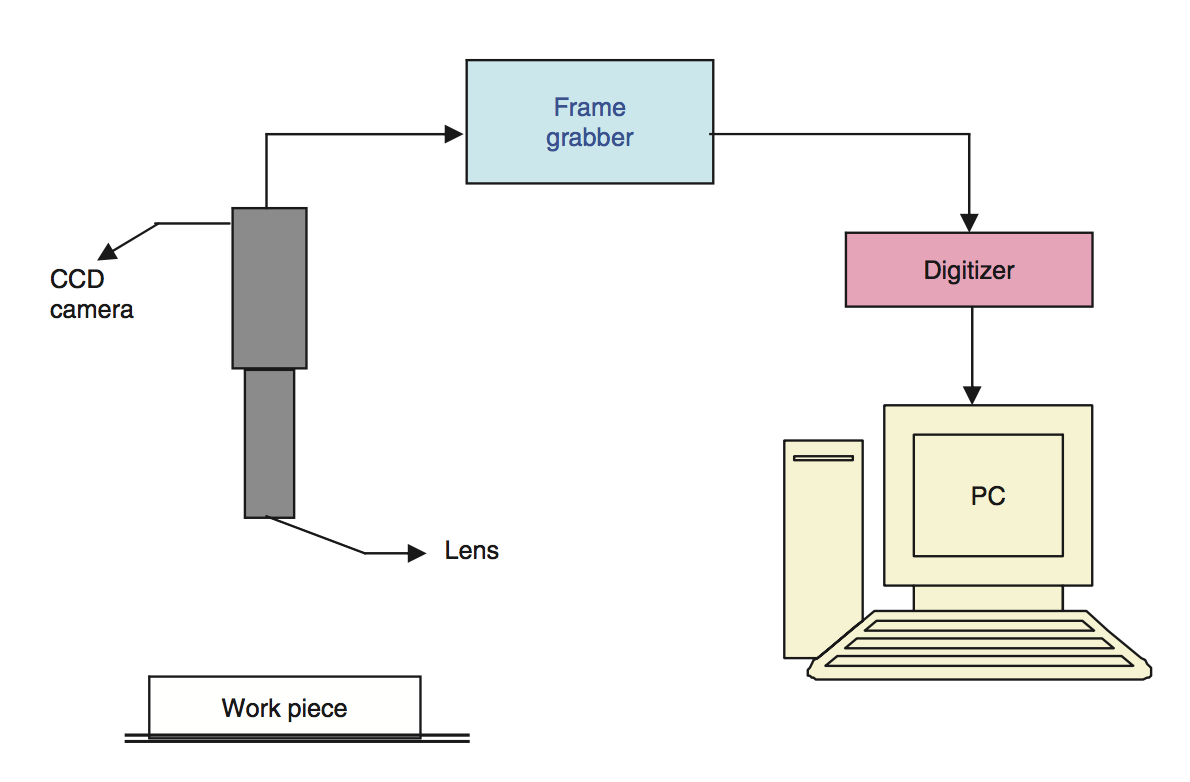
\includegraphics[scale=0.6]{Imagens/imgPro.png}
	\caption{Diagram of a machine vision system \cite{sarma2009surface}}
	\label{fig:imgProcessing}
\end{figure}

There are many applications for image processing in the machining industry. \citeonline{sarma2009surface} developed a method for roughness determination ($R_{a}$), correlating gray scaled images with surface finish of glass fiber reinforced polymer (GFRP). After GFRP machining, images of the workpiece were taken by means of charge couple device camera and then processed (figure \ref{fig:imgProcessing}), obtaining a significant correlation between the predicted and real roughness.

\citeonline{jeon1988optical} and \citeonline{kurada1997machine} also developed an image processing method to monitor flank wear of cutting tools \emph{in situ}. Images in grayscale were taken and consequently processed for boundaries extraction, which indicates wear areas on tool tip surroundings.

Also, \citeonline{khalifa2006image} presented a method for chatter identification in turning processes, which is a significant challenge when comes to automatic machining processes. The vision system compares surface finish of workpieces machined under chatter and chatter-free conditions by means of roughness parameter. The method is also based on the behavior and distribution of gray levels in images of the workpiece.

 These are a few examples of what image processing can do for machining industry. There are uncountable other ways in which it can be applied to improve processes and quality of final products. The fast development of computer hardware makes the processing time of images continuously shorter, allowing vision systems to be incorporated in online monitoring and providing real time feedback.